\subsection{IRS observations}
\label{sect:irs_obs}

% SPW: Fig 1: label F_nu(8 \micron), etc., not just "8/24".
\begin{figure}
\centering
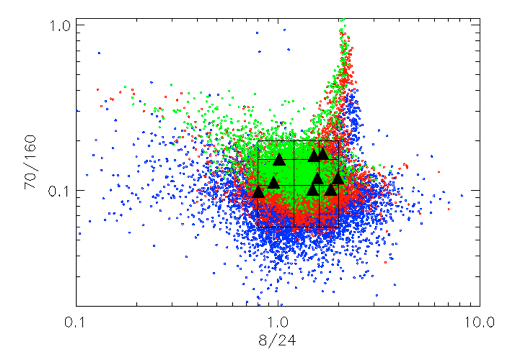
\includegraphics[width = 8 cm]{./colormaps.png}
\caption{$8 - 24/70 - 160$ $\mu$m colour-colour diagram of M31 obtained from IRAC and MIPS. The plot is divided into 9 regions (black grid) and the observations were made to cover those regions. The triangles indicate the regions we observed. ({\bf Needs a better explanation} )}
\label{colourmaps}
\end{figure}

We obtained mid-infrared spectral maps of 12 regions in M31 using the {\em Spitzer}/IRS instrument \citep{IRS2004} covering wavelengths from 5 to 21 microns. 
These regions include the nucleus, two regions previously observed by ISOCAM, and 9 other regions chosen to cover a range of UV intensities, 
metallicities and dust temperatures. Dust temperatures were determined using an $8 - 24/70 - 160$ $\mu$m colour-colour diagram 
(see Figure~\ref{colourmaps}). The locations of the observed regions are shown in Figure~\ref{m31}, and 
their coordinates are given in Table~\ref{regions}. The two regions previously observed by ISOCAM are the region from the bulge and the 
region from the active region in the star-forming ring (Region 9 in our sample). A background observation was also made off the galaxy 
along the minor axis and it was used to enable the background subtraction from the data cubes.

%MLNA: Table 1 would be better if it included the galactocentric radii (perhaps), and the UV intensities, metallicities, and dust temperatures (definitely) used to choose them as targets in the first place.  
%SPW: As to tables, I'd consolidate 1, 2, and 5 into a single table.  Add rows as appropriate for "nucleus" and "north", and give their dimensions in a footnote.  
\begin{table*}
 \centering
 \begin{minipage}{90mm}
\caption{Spitzer/IRS Target Locations in M31
\label{regions}}
\begin{tabular}{lccrl}
\hline Name & R.A. (J2000) & Decl. (J2000) & ${R_{\rm gc}}^b$ & $12+\log({\rm O/H})$
\\
 \hline
Nucleus$^a$ & $00^{\rmn{h}}42^{\rmn{m}}44\fs31$ & $41\degr16\arcmin09\farcs4$  & 0.0 & \\
Bulge$^a$   & $00^{\rmn{h}}42^{\rmn{m}}35\fs00$ & $41\degr21\arcmin01\farcs0$  & 4.7 &$8.90\pm0.03$\\
Region 1    & $00^{\rmn{h}}41^{\rmn{m}}30\fs41$ & $40\degr43\arcmin07\farcs8$  & 12.4 &$9.20\pm0.20$\\
Region 2    & $00^{\rmn{h}}45^{\rmn{m}}22\fs85$ & $41\degr38\arcmin53\farcs1$  & 13.0 &$9.07\pm0.02$\\
Region 3    & $00^{\rmn{h}}40^{\rmn{m}}37\fs37$ & $41\degr01\arcmin29\farcs4$  & 12.1 &$8.85\pm0.01$\\
Region 4    & $00^{\rmn{h}}41^{\rmn{m}}17\fs86$ & $41\degr07\arcmin09\farcs8$  & 8.7 &$8.89\pm0.06$\\
Region 5    & $00^{\rmn{h}}43^{\rmn{m}}39\fs57$ & $41\degr19\arcmin03\farcs1$  & 7.0 &$8.93\pm0.08^c$\\
Region 6    & $00^{\rmn{h}}43^{\rmn{m}}35\fs72$ & $41\degr23\arcmin15\farcs0$  & 4.3 &$8.73\pm0.08$\\
Region 7    & $00^{\rmn{h}}40^{\rmn{m}}53\fs98$ & $40\degr58\arcmin58\farcs9$  & 8.7 &$8.40\pm0.08$\\
Region 8    & $00^{\rmn{h}}42^{\rmn{m}}21\fs60$ & $41\degr07\arcmin17\farcs4$  & 3.1 &$8.94\pm0.08^c$\\
Region 9$^a$& $00^{\rmn{h}}41^{\rmn{m}}00\fs00$ & $40\degr36\arcmin20\farcs3$  & 13.5 &$8.86\pm0.02$\\
NGC~206     & $00^{\rmn{h}}40^{\rmn{m}}20\fs20$ & $40\degr44\arcmin54\farcs0$  & 9.8 & \\
Background  & $00^{\rmn{h}}44^{\rmn{m}}41\fs80 $ & $40\degr58\arcmin56\farcs0$  & 29.5 & \\
\hline
\end{tabular}
{$^a$Regions with ISOCAM data.\\
$^b$De-projected galactocentric distance, in kpc\\ 
$^c$Metallicities obtained from the radial metallicity profile of M31.}
\end{minipage}
\end{table*}

\begin{figure*}
\centering
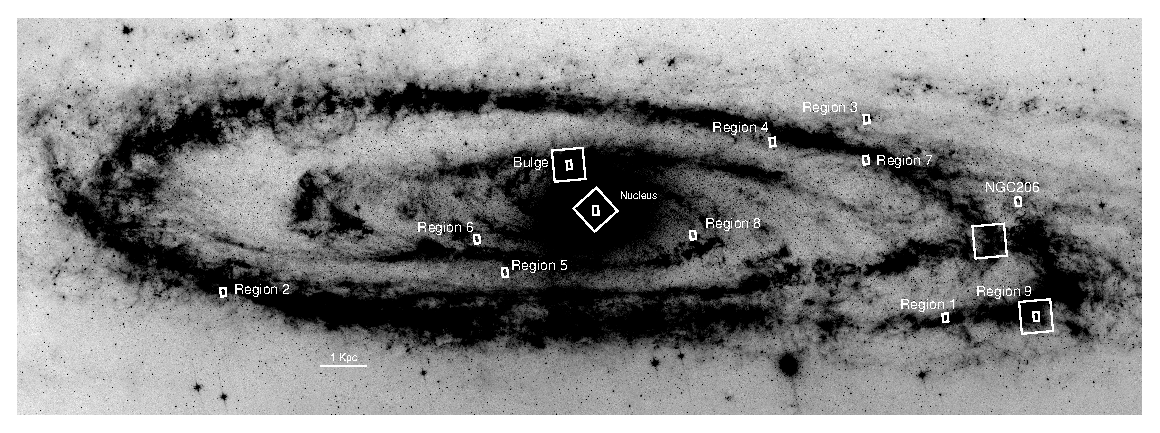
\includegraphics[scale=0.9]{./m31_map.eps}
\caption{An 8 micron IRAC image of M31 \citep{Barmby2006lr}. Small white rectangles ($30\arcsec\times50\arcsec$) show the regions that we observed and larger squares ($192\arcsec\times192\arcsec$) show the regions observed by  \citet{1998Cesarsky}.
\label{m31}
}
\end{figure*}


For our observations we used the IRS Short-Low (SL) and Long-Low (LL) modules which cover wavelengths from 5 to 21 microns. 
The Low modules have resolving power in the range 60--130. Each low-resolution module is divided into two sub-slits 
which provide spectroscopy in either first or second order. They are denoted as SL1 (7.5--14.5~$\mu$m), SL2 (5.2--7.6~$\mu$m),
LL1 (20.5--38.5~$\mu$m, not used in these observations), and LL2 (14.5--20.75~$\mu$m).
All M31 regions were observed in September 2007 as part of G. G. Fazio's Guaranteed Time (program ID 40032). 
The map size was based on the size 
of the IRS slits (SL: $3.6\arcsec \times 57\arcsec$, LL: $10.5\arcsec \times 168\arcsec$). Each region was covered by 18 overlapping observations 
of the SL slit and 11 overlapping observations of the LL slit making the map size $32\arcsec \times 57\arcsec$ for SL and $58\arcsec \times 168\arcsec$ for LL. 
Figure~\ref{slits} shows an example of the slit arrangement. For the brighter regions (nucleus, bulge), ramp times of 14 s (SL) and 30 s (LL) were used, 
while for the fainter regions, ramp times of 60 and 120 s were used respectively. Background observations were taken with each module (2 per ramp time). 
Since all of the targets are in the same part of the sky, a common background observation was used for multiple targets to subtract the background emission. 

% PB: for Dimuthu to do: remake figure to drop second black box
\begin{figure}
\centering
\includegraphics[scale=0.3]{./cubeslits.eps}
\caption{SL1 data cube from the nucleus showing the arrangement of slits used to cover the region. 
A black box outlines the footprint of the short-low maps and the green box outlines the LL2. Blue and red slits show how 
each map was covered using overlapping slit positions.
\label{slits}
}
\end{figure}

\subsection{IRS Data Reduction}

The data were reduced through the SSC pipeline (ver. S17.2.0) and the maps were assembled using the CUBISM program \citep{Smith:2007fk}. 
Bad pixel removal was also done using CUBISM and the background observations were used to subtract the background emission from these cubes 
following the method outlined in \citet{Gordon:2008lr}. Spectra were extracted using a $30\arcsec\times50\arcsec$   rectangular aperture,
which corresponds to $114\times190$~pc at the distance of M31.
The aperture size was selected to cover the overlapping area of the SL and LL modes; all the IRS maps cover additional area than is considered here.
The spectrum from the NGC 206 is very noisy and was removed from our analysis. 


There is wavelength overlap between the SL1 and SL2 spectra, and between SL1 and LL2;
to generate a single spectrum for each M31 region it is necessary to combine the spectra and
account for photometric offsets between them. We first combined the extracted SL1 and SL2 
spectra by computing the average flux densities over the wavelength overlap region ($7.5 < \lambda< 7.6\mu$m),
adding a constant  to the SL2 spectra so that they matched the SL1 average,
and averaging the SL1 $+$ shifted SL2 spectra over the overlap region.
After this procedure there was still a noticeable mis-match between the SL and LL spectra. We addressed this
by scaling the SL spectra to match IRAC 8~$\mu$m fluxes as follows. IRAC fluxes were measured
on the 8~$\mu$m image \citep{Barmby2006lr} in the same apertures used to extract the IRS spectra
and the extended source  aperture correction of 0.824 applied.
Uncertainties on these measurements were estimated as the standard deviation of the measured
IRAC flux in a similarly-sized region off the disk of the galaxy ($00^{\rmn{h}}48^{\rmn{m}}58\fs0, +42\degr14\arcmin54\farcs0$). 
The {\em Spitzer} synthetic photometry software \citep{SpitzerDAC} 
was then used to quantify the colour correction for each spectrum, i.e. the
multiplicative factor $K$ between the IRAC photometry over its broad bandpass and the IRS flux
density at the centre of the bandpass. The IRAC photometry, IRS flux density, and colour corrections 
for each region are given in Table~\ref{colourK}. Plotting the IRS  and colour-corrected IRAC measurements
(Figure~\ref{offset}) and fitting a straight line weighted by the uncertainties, we found that the best-fit relation 
between the measurements had a slope of $0.81\pm0.08$  and intercept of $-0.05\pm0.06$. 
The non-zero intercept of this fit suggested that an additive offset was more appropriate for combining SL and LL
spectra than a multiplicative one; this method was also used by \citet{Gordon:2008lr} and \citet{Engelbracht_2008}.
Therefore we scaled each SL spectrum by an offset 
\begin{equation}
x = F_{\rm IRAC8}/K -   F_{\rm IRS8}.
\label{eq:offset}
\end{equation}
The scaled SL spectra were much better matched to the LL spectra, and the final combination
of SL and LL was done using the average-and-offset procedure described above for SL1 and SL2.


\begin{table}
 \centering
 \begin{minipage}{100mm}
\caption{Matched aperture photometry}
  \begin{tabular}{lcccc}
  \hline{Name}&{IRS$^{a}$}&{IRAC$^{b}$}&{$K^{\rm c}$}&{Offset $x^d$} \\ 
{} & { MJy~sr$^{-1}$} & { MJy~sr$^{-1}$} & &  MJy~sr$^{-1}$
   \\
 \hline
 Region 1 & 1.8505 & 1.3923 & 0.532 & 0.3061
 \\ Region 2  & 1.8238 & 1.3731 & 0.555 & 0.2148
 \\ Region 3 & 0.7192 & 0.9689 & 0.767 & 0.3218
 \\ Region 4 & 1.1431 & 0.8513 & 0.589 & 0.0407
 \\  Region 5 & 0.6787 & 0.8088 & 0.773 & 0.1834
 \\  Region 6  & 0.6399 & 0.7656 & 0.927 & 0.0479
 \\  Region 7  & 1.1538 & 0.8243 & 0.526 & 0.1380
 \\ Region 8 & 0.5556 & 0.7135 & 0.877 & 0.1148
 \\  Region 9 & 1.9413 & 1.6562 & 0.606 & 0.3107 
 \\ Bulge & 2.6956 & 2.5473 & 0.532 & 1.2425\\
\hline
 \label{colourK}
\end{tabular}\\
 {$^{\rm a}$Specific intensity measured at 8.00~$\mu$m, no colour correction.\\
 $^{\rm b}$Specific intensity measured over the IRAC 8~$\mu$m bandpass,\\ no extended source correction.\\
$^{\rm c}$Colour correction factor computed from IRS spectrum\\
 $^{\rm d}$Computed offset between IRAC and IRS as defined in~Eq.~\ref{eq:offset}. }
\end{minipage}
\end{table}

	
\begin{figure}
\centering
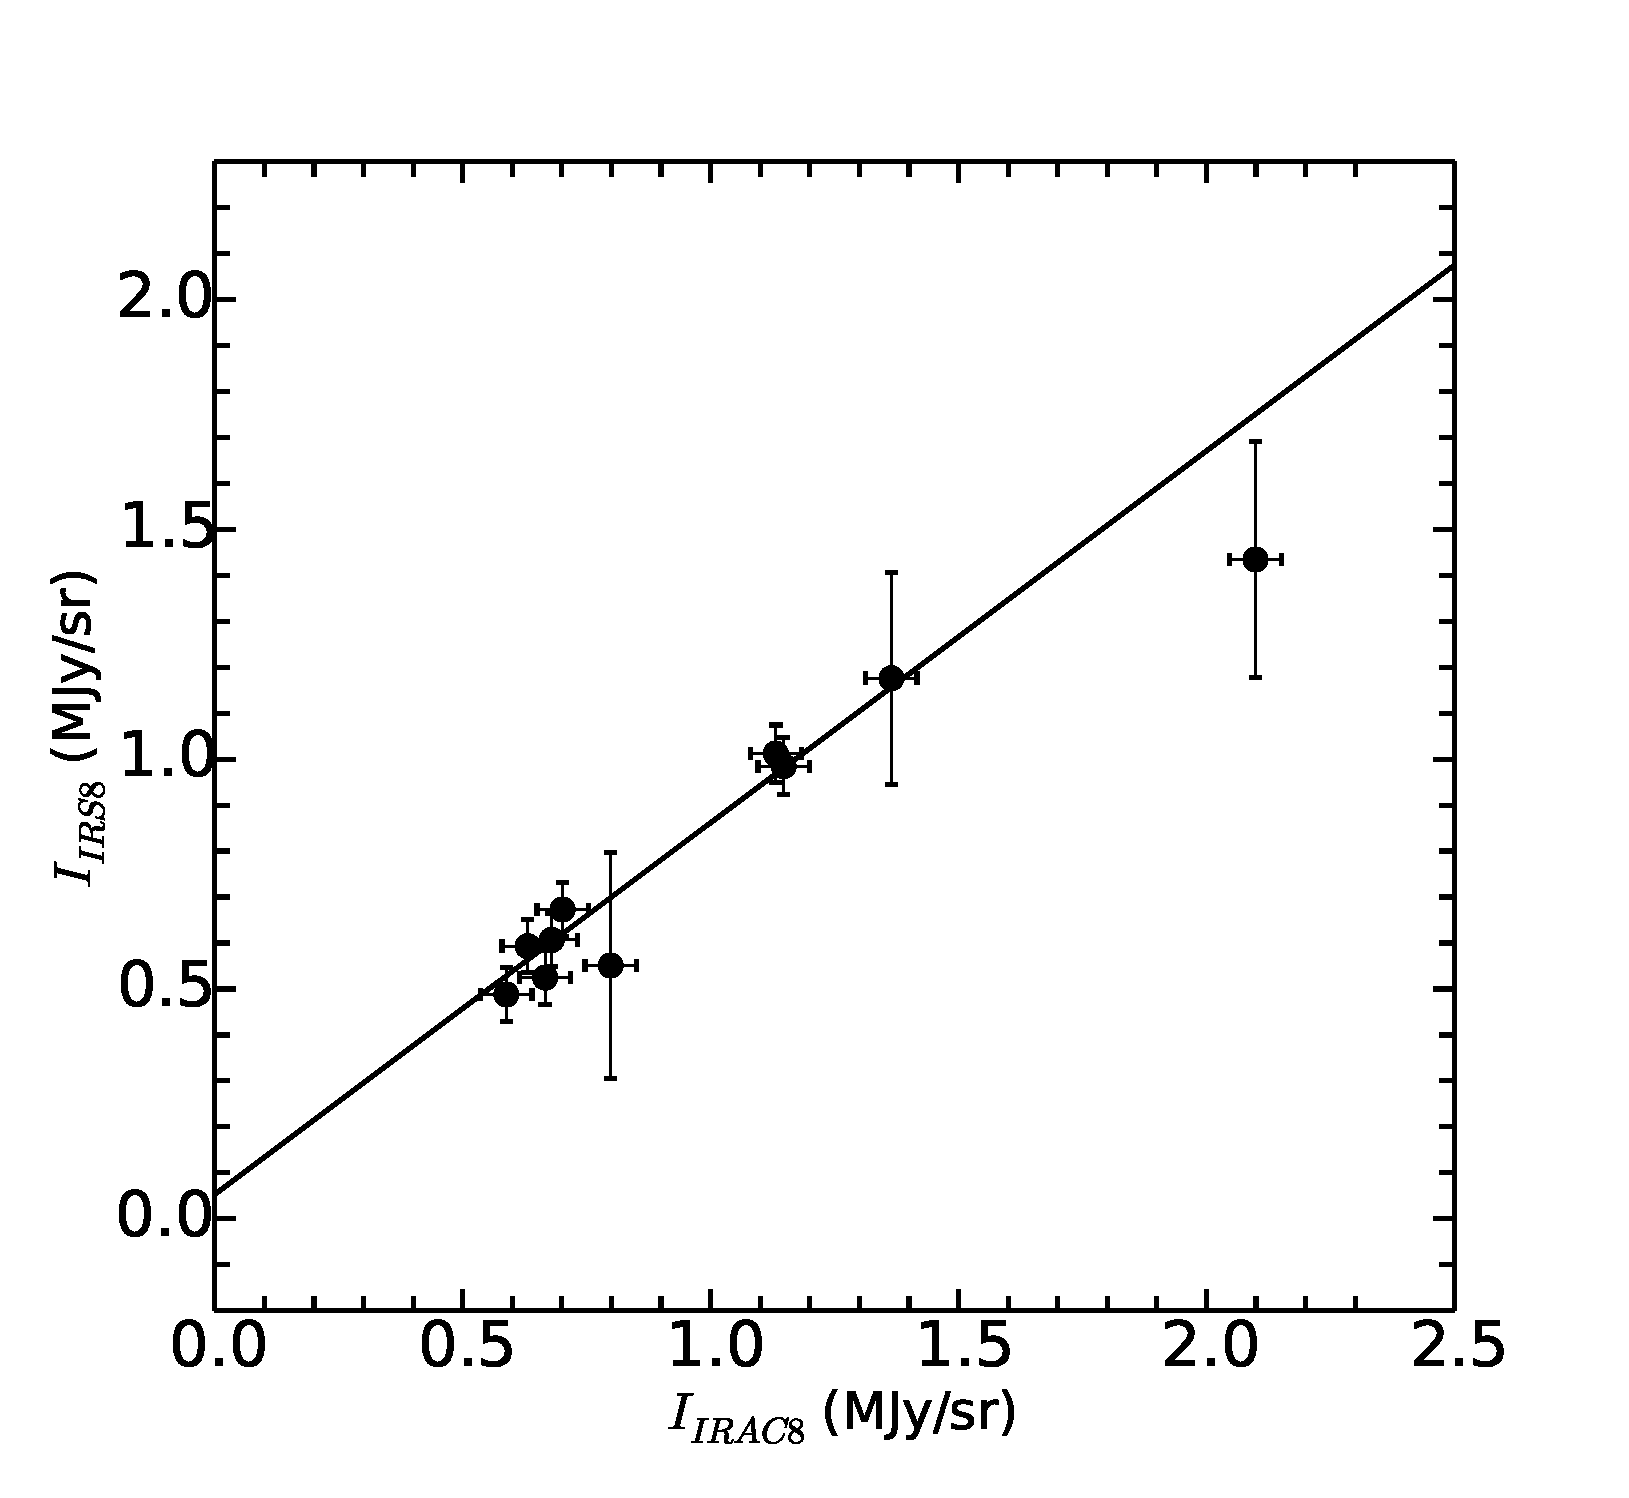
\includegraphics[scale=0.25]{./offset.eps}
\caption{ Intensity of the aperture corrected IRAC 8~$\mu$m image vs that of the colour corrected IRS spectra at 8~$\mu$m  obtained using the same aperture for our regions in M31. The straight line is the line of best fit. }
\label{offset}
\end{figure}

% TODO: tables need some reformatting, such as $x\pm y$

\begin{table*}
 \centering
 \begin{minipage}{200mm}
\caption{PAH Emission Line Strengths$^a$}
  \begin{tabular}{l c c  c  c  c  c  c  c  c  c c }
  \hline {Region  }&{5.7$\mu$m  }&{6.2$\mu$m  }&{7.7$\mu$m  }&{8.3$\mu$m  }&{8.6$\mu$m  }&{10.7$\mu$m  }&{11.3$\mu$m  }&{12.0$\mu$m  }&{12.7$\mu$m  }&{17.0$\mu$m  } 
   \\
 \hline
 Region 1 &10$\pm$1            & 34$\pm$1-09        & 107$\pm$10        & 13$\pm$1       & 14.1$\pm$0.9        & 2.2$\pm$0.3        & 33.4$\pm$0.9        & 9.1$\pm$0.5        & 16$\pm$1        & 17$\pm$1        \\
Region 2 &7.7$\pm$0.9        & 31.2$\pm$0.8        & 106$\pm$8        & 9$\pm$1           & 19.8$\pm$0.8        & 1.5$\pm$0.2        & 32.0$\pm$0.8        & 6.6$\pm$0.4        & 15$\pm$1        & 14.7$\pm$0.9        \\
Region 3 &8$\pm$4              & 25$\pm$3                & 111$\pm$22       & 21$\pm$4       & 7$\pm$3                 & 1.1$\pm$0.9        & 19$\pm$3             & 6$\pm$1             & 14$\pm$3           & 13$\pm$2        \\
Region 4 &4$\pm$1              & 15.8$\pm$0.9        & 59$\pm$9        & 7$\pm$1           & 11.6$\pm$0.8          & 0.8$\pm$0.2        & 19.9$\pm$0.8        & 3.5$\pm$0.4        & 9$\pm$1             & 12.5$\pm$0.9        \\
Region 5 &1$\pm$1              & 7$\pm$1                 & 22$\pm$3        & 3$\pm$1           & 5.8$\pm$0.8            & 0.9$\pm$0.2        & 12.7$\pm$0.8        & 2.4$\pm$0.4        & 6.3$\pm$0.4        & 10$\pm$2        \\
Region 6 & - - - -                      & 7.3$\pm$0.9         & 22$\pm$7        & 3$\pm$1            & 3.6$\pm$0.8            & 0.8$\pm$0.2        & 10.8$\pm$0.8        & 1.9$\pm$0.4        & 4.5$\pm$0.4        & 8.3$\pm$0.6        \\
Region 7 &5.9$\pm$0.9        & 17.7$\pm$0.9       & 57$\pm$8        & 9$\pm$1            & 12.8$\pm$0.8        & 1.6$\pm$0.2        & 21.8$\pm$0.8        & 5.2$\pm$0.4        & 11$\pm$1             & 13$\pm$2        \\
Region 8 &2.$\pm$1              & 3$\pm$1              & 6$\pm$3            & 3$\pm$1            & 2.7$\pm$0.8        & 1.4$\pm$0.3        & 4.4$\pm$0.8            & - - - -                      &  - - - -                       & 4.1$\pm$0.7        \\
Region 9 &  - - - -                     & 38$\pm$3          & 133$\pm$29        & 25$\pm$4        & 15$\pm$3            & 2.4$\pm$0.8        & 37$\pm$3               & 14$\pm$1             & 25$\pm$3        & 19$\pm$6        \\
Bulge       & - - - -                       & 38$\pm$2           & 219$\pm$27        & 32$\pm$4        & 20$\pm$3           & 2.0$\pm$0.9        & 53$\pm$3              & 14$\pm$1           & 29$\pm$3        & 39$\pm$2       \\
\hline
 \label{PAHlinetable}
\end{tabular}\\
{$^a$Units are 10$^{-9}$~W~m$^{-2}$.}
\end{minipage}
\end{table*}







\begin{table*}
 \centering
 \begin{minipage}{200mm}
\caption{PAH Emission Line Equivalent Widths$^a$}
  \begin{tabular}{l c c  c  c  c  c  c  c  c  c c }
  \hline {Name  }&{5.7$\mu$m  }&{6.2$\mu$m  }&{7.7$\mu$m  }&{8.3$\mu$m  }&{8.6$\mu$m  }&{10.7$\mu$m  }&{11.3$\mu$m  }&{12.0$\mu$m  }&{12.7$\mu$m  }&{17.0$\mu$m  } 
   \\
 \hline
 Region 1 &0.39$\pm$0.08        & 1.2$\pm$0.1             & 3.4$\pm$0.3        & 0.43$\pm$0.04        & 0.47$\pm$0.04        & 0.09$\pm$0.01        & 1.45$\pm$0.04        & 0.43$\pm$0.03        & 0.78$\pm$0.03              & 1.27$\pm$0.05        \\
 Region 2 &0.28$\pm$0.04        & 1.02$\pm$0.06        & 3.4$\pm$0.2        & 0.32$\pm$0.04        & 0.70$\pm$0.04        & 0.07$\pm$0.01        & 1.58$\pm$0.04        & 0.35$\pm$0.02        & 0.85$\pm$0.03              & 1.35$\pm$0.06        \\
 Region 3$^b$ &4$\pm$2           & 8$\pm$2                   & 19$\pm$4            & 2.8$\pm$0.8             & 0.9$\pm$0.5             & 0.1$\pm$0.1            & 2.1$\pm$0.3             & 0.7$\pm$0.2            & 1.6$\pm$0.2                   & 2.4$\pm$0.3        \\
 Region 4 &0.28$\pm$0.09        & 1.0$\pm$0.1             & 3.7$\pm$0.4       & 0.5$\pm$0.1              & 0.77$\pm$0.07        & 0.07$\pm$0.02        & 1.67$\pm$0.06        & 0.31$\pm$0.04        & 0.86$\pm$0.05             & 1.68$\pm$0.07        \\
 Region 5 & - - - -        & 0.12$\pm$0.03        & 0.61$\pm$0.08   & 0.10$\pm$0.03        & 0.20$\pm$0.03        & 0.05$\pm$0.01        & 0.77$\pm$0.03        & 0.17$\pm$0.03        & 0.50$\pm$0.04            & 1.6$\pm$0.2        \\
 Region 6 & - - - -                          & 0.10$\pm$0.04        & 0.6$\pm$0.2        & 0.10$\pm$0.04        & 0.14$\pm$0.03        & 0.05$\pm$0.01        & 0.77$\pm$0.04        & 0.15$\pm$0.03        & 0.42$\pm$0.04            & 1.7$\pm$0.1        \\
 Region 7 &0.32$\pm$0.05        & 0.86$\pm$0.06        & 2.8$\pm$0.2        & 0.44$\pm$0.06        & 0.69$\pm$0.06        & 0.12$\pm$0.02        & 1.81$\pm$0.07        & 0.48$\pm$0.05        & 1.11$\pm$0.08            & 2.2$\pm$0.2        \\
 Region 8 &0.03$\pm$0.04        & 0.04$\pm$0.03        & 0.2$\pm$0.10      & 0.09$\pm$0.04        & 0.10$\pm$0.03        & 0.09$\pm$0.02        & 0.30$\pm$0.02        & 0.00$\pm$0.00        & 0.01$\pm$0.01            & 0.62$\pm$0.07        \\
 Region 9$^b$ & - - - -                 & 237$\pm$100          & 151$\pm$60        & 16$\pm$6                 & 8$\pm$3                   & 0.5$\pm$0.2             & 7$\pm$1                   & 2.3$\pm$0.6             & 3.6$\pm$0.8                 & 2.4$\pm$0.8  \\
 Bulge       & - - - -                          & 1.2$\pm$0.2            & 4.0$\pm$0.4        & 0.51$\pm$0.07         & 0.30$\pm$0.06        & 0.03$\pm$0.01        & 0.78$\pm$0.03        & 0.22$\pm$0.02        & 0.49$\pm$0.03            & 1.16$\pm$0.04 \\       
\hline
 \label{EQW}
\end{tabular}\\
{$^a$Units are $\mu$m. 
$^b$Continuum for these regions is very weak.  Equivalent widths are highly uncertain and not considered in the analysis (see Section~\ref{sect:data_analysis}).}
\end{minipage}
\end{table*}


\begin{table*}
 \centering
 \begin{minipage}{100mm}
\caption{Atomic Emission Line Strengths$^a$}
  \begin{tabular}{l c c  c  c  c  c  }
  \hline{Name  }&{[Ar~{\sc ii}] }&{[Ar~{\sc iii}]  }&{[S~{\sc iv}]}&{[Ne~{\sc ii}]   }&{[Ne~{\sc iii}]   }&{[S~{\sc iii}]  }\\
{}&{\tiny{7.0$\mu$m} }&{\tiny{9.0$\mu$m }}&{\tiny{10.5$\mu$m}}&{\tiny{12.8$\mu$m  }}&{\tiny{15.5$\mu$m } }&{\tiny{18.7$\mu$m }} 
   \\
 \hline 
 
Region 1 &    $<$15.2                 & $<$16.4                 & 6$\pm$1                 & 6$\pm$1                 & $<$ 4.2                 & 2.2$\pm$0.4                \\
Region 2 &    5$\pm$3                 & $<$ 17.4               & $<$5.1                    & 6$\pm$1                 & $<$ 2.9                 & 0.9$\pm$0.5                 \\
Region 3 &    $<$42.9                 & 27$\pm$6              & $<$ 28.9                & 9$\pm$3                 & 6$\pm$1               & 4.3$\pm$0.9                 \\
Region 4 &    $<$11.2                 & $<$10.0                 & $<$4.4                    & 2$\pm$1                 & 0.6$\pm$0.5        & 1.3$\pm$0.5                 \\
Region 5 &    4$\pm$3                 & $<$6.2                   & $<$ 5.2                 & $<$ 4.2                     & 2$\pm$1               & 2$\pm$1                 \\
Region 6 &    7$\pm$3                & 4$\pm$2                 & $<$ 3.8                 & 2$\pm$1                  & 5.4$\pm$0.5         & 5.3$\pm$0.5                 \\
Region 7 &    3$\pm$3                 & $<$12.6                 & 2.3$\pm$0.9        & 10$\pm$2                & $<$ 2.9                 & 8$\pm$1                \\
Region 8 &    $<$11.8                  & 5$\pm$2                & $<$4.9                  & $<$2.6                       & 11.6$\pm$0.5     & 6.5$\pm$0.5                 \\
Region 9 &    24$\pm$10             & 35$\pm$8             & $<$ 2.7                 & 38$\pm$3                 & 7$\pm$4               & 15.3$\pm$5.6                 \\
Bulge &          10$\pm$7               & 49$\pm$7              & $<$ 30.4               & 19$\pm$4                 & 7$\pm$2               & 2$\pm$1      \\           

\hline
 \label{Atomic}
\end{tabular}\\
{ $^a$Units are 10$^{-10}$~W~m$^{-2}$. Upper limits are indicated with a $<$ mark.  }
%SPW: Table 4: units of 10^-10 W m^-2 must be wrong.  I'd expect 10^-15 or so.
%SPW: How many sigma are the upper limits?

\end{minipage}
\end{table*}



\subsection{ISOCAM Data Reduction}
\label{sect:iso_data}

To compare our results with those of  \citet{1998Cesarsky}, we retrieved the highly processed ISOCAM data provided by \citet{Boulanger_F_2005}  
for the three regions in common. 
The ISOCAM data were obtained with the circular variable filters (CVFs) over a $3\arcmin \times 3\arcmin$ field of view at a scale of 6\arcsec\ per pixel. 
The wavelength range covered was 5.15--16.5~$\mu$m at a resolution of $\lambda/\Delta \lambda \approx 45$; the ISOCAM instrument is described by \citet{cesarsky1996}.
An image of the ISOCAM data is shown in Figure~\ref{isonuc}.  For the three regions, we extracted spectra using the same 
$30\arcsec\times50\arcsec$ aperture as for the IRS data. 

% SPW: Fig 5: mention "negative image" (if that's what it is).  Also mention spectral band of image.
\begin{figure}
\centering
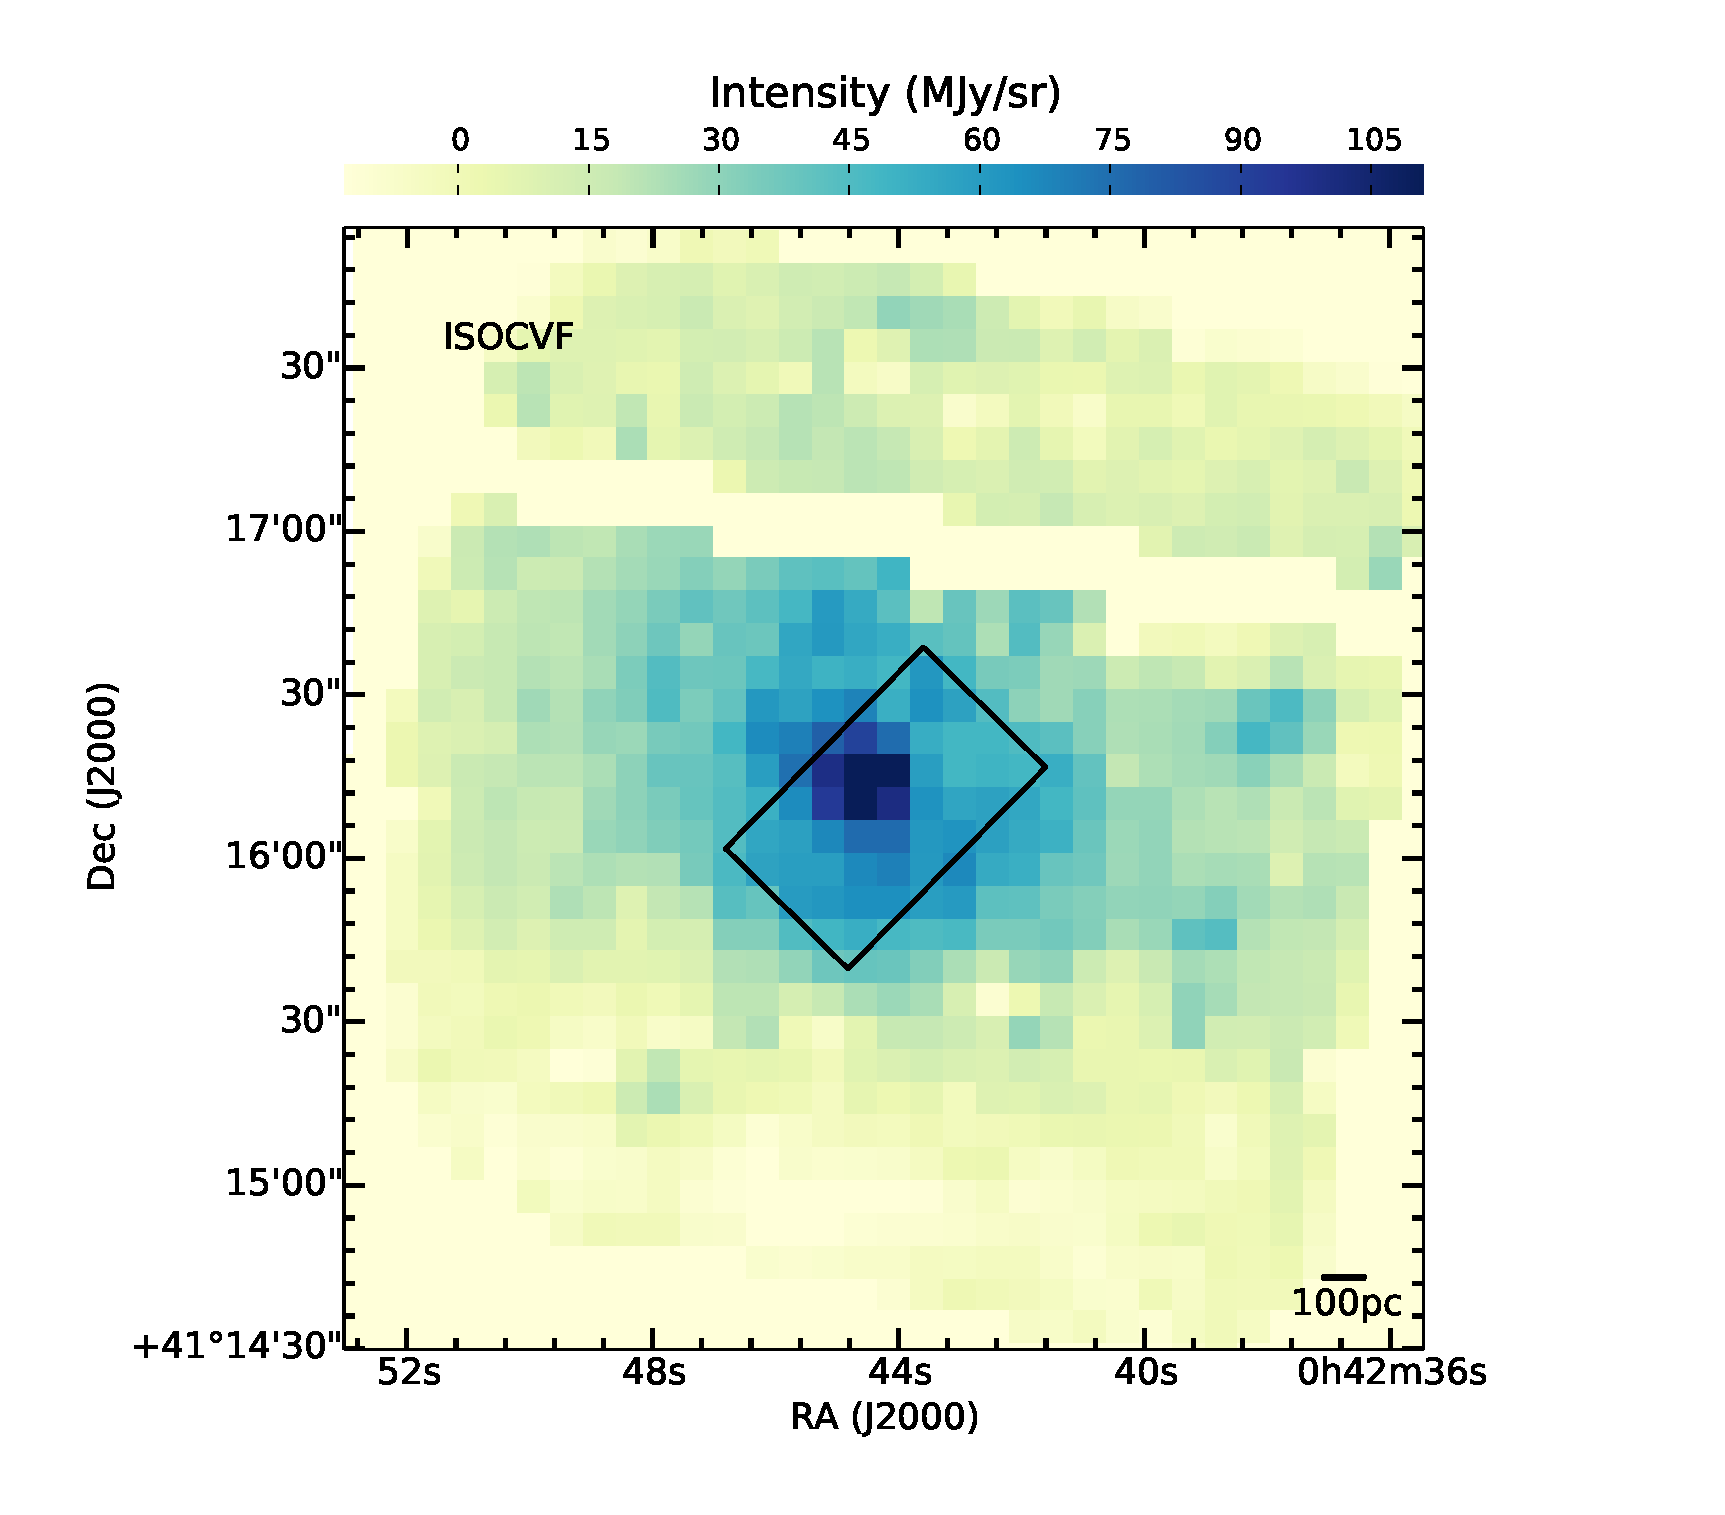
\includegraphics[width = 8cm]{./isonuc.eps}
\caption{11.3~$\mu$m negative image of the ISOCAM data cube from the nucleus of M31. The black box shows the size of the aperture ($30\arcsec\times50\arcsec$) used to extract spectra.}
\label{isonuc}
\end{figure}
